\documentclass{beamer}
\usetheme{Boadilla} 
\setbeamercovered{invisible}
\setbeamertemplate{navigation symbols}{} 
%\useoutertheme{infolines} 

\usepackage[utf8]{inputenc}
\usepackage{graphicx}

\setbeamertemplate{frametitle continuation}{} 
\usepackage{subfigure}
\usepackage{caption}
\usepackage{bm}
\usepackage{epsfig}

\usepackage{amsmath}
\usepackage{xcolor,colortbl}

\usepackage{multicol}
\usepackage{wasysym}

\usepackage{hyperref}
\usepackage{float}

\usepackage{array}
\newcolumntype{L}[1]{>{\raggedright\let\newline\\\arraybackslash\hspace{0pt}}m{#1}}
\newcolumntype{C}[1]{>{\centering\let\newline\\\arraybackslash\hspace{0pt}}m{#1}}
\newcolumntype{R}[1]{>{\raggedleft\let\newline\\\arraybackslash\hspace{0pt}}m{#1}}

\usepackage[T1]{fontenc}
\usepackage{tikz}
\usetikzlibrary{shadows}

\newcommand*\keystroke[1]{%
  \tikz[baseline=(key.base)]
    \node[%
      draw,
      fill=white,
      drop shadow={shadow xshift=0.25ex,shadow yshift=-0.25ex,fill=black,opacity=0.75},
      rectangle,
      rounded corners=2pt,
      inner sep=1pt,
      line width=0.5pt,
      font=\scriptsize\sffamily
    ](key) {#1\strut}
  ;
}

% deal with spaces in absolute paths

\usepackage[space]{grffile}
\graphicspath{{C:/Users/Yered/Dropbox/Harvard/Winter 2014/CdeC/Slides/Introduction/figures/}}

\usepackage[scaled]{helvet}
\usepackage[round]{natbib}


\begin{document}
\title[Datos de Expresi\'{o}n Gen\'{e}tica]{Explorando el Transcriptoma con Datos de Expresi\'{o}n Gen\'{e}tica\\
\vspace{0.5cm}
Datos de Expresi\'{o}n Gen\'{e}tica}
\author{Yered Pita-Ju\'{a}rez}
\institute[CdeC M\'{e}rida]{}
\date{6/1/2015}


\begin{frame}
\titlepage
\end{frame}


\begin{frame}{Datos de Microarreglos}
\begin{itemize}
\item Muestra de ARN preparada, etiquetada e hibridizada al microarreglo
\item El escáner genera una imagen (\texttt{.DAT})
\item Se separan los pixeles por sonda
\item La intensidad luminosa se promedia por sonda (\texttt{.CEL})
\end{itemize}
\end{frame}

\begin{frame}[fragile]{Datos de Microarreglos}
\begin{itemize}
\item Descarga y extrae los estos archivos en tu working directory\\
\url{https://www.dropbox.com/s/qeg81zxoxfzjknr/celfiles.zip}
\item working directory
\begin{verbatim}
wd <- getwd()
basedir <- paste0(wd, "/celfiles")
setwd(basedir)
\end{verbatim}
\item Primero vamos a extraer la información acerca de estas muestras
\begin{verbatim}
library(affy)
tab <- read.delim("sampleinfo.txt",
				   check.names=FALSE,as.is=TRUE)
rownames(tab) <- tab$filenames
tab
\end{verbatim}
\end{itemize}
\end{frame}

\begin{frame}[fragile]{Datos de Microarreglos}
\begin{itemize}
\item Vamos a ver que archivos \verb=CEL= estan disponibles
\begin{verbatim}
fns <- list.celfiles()
fns
\end{verbatim}
\item ¿Tenemos todos los archivos?
\begin{verbatim}
fns %in% tab[,1]
\end{verbatim}
\item Vamos a crear un objecto AffyBatch incluyendo la informacion provista acerca de estas muestras
\begin{verbatim}
ab <- ReadAffy(phenoData=tab)
dim(pData(ab))
\end{verbatim}
\item ¿Que plataforma?
\begin{verbatim}
annotation(ab)
\end{verbatim}
\item Affymetrix Human Genome U95 (\texttt{hgu95a})
\end{itemize}
\end{frame}


\begin{frame}[fragile]{Procesando los Datos}
\textbf{Robust Multichip Average (RMA)}
\begin{enumerate}
\item Corrección de fondo
\item Normalización
\item Resumen
\end{enumerate}
\textbf{Corrección de fondo}
\begin{itemize}
\item Observado = Señal + Fondo
\item Nos interesa la señal
\item Estimar la señal usando métodos de inferencia estadística
\end{itemize}
\end{frame}


\begin{frame}[fragile]{Procesando los Datos}
\textbf{Normalización}
\begin{itemize}
\item Ajustar las mediciones de los arreglos para que esten en la misma escala
\item Poder comparar las muestras
\begin{figure}[H]
\centering
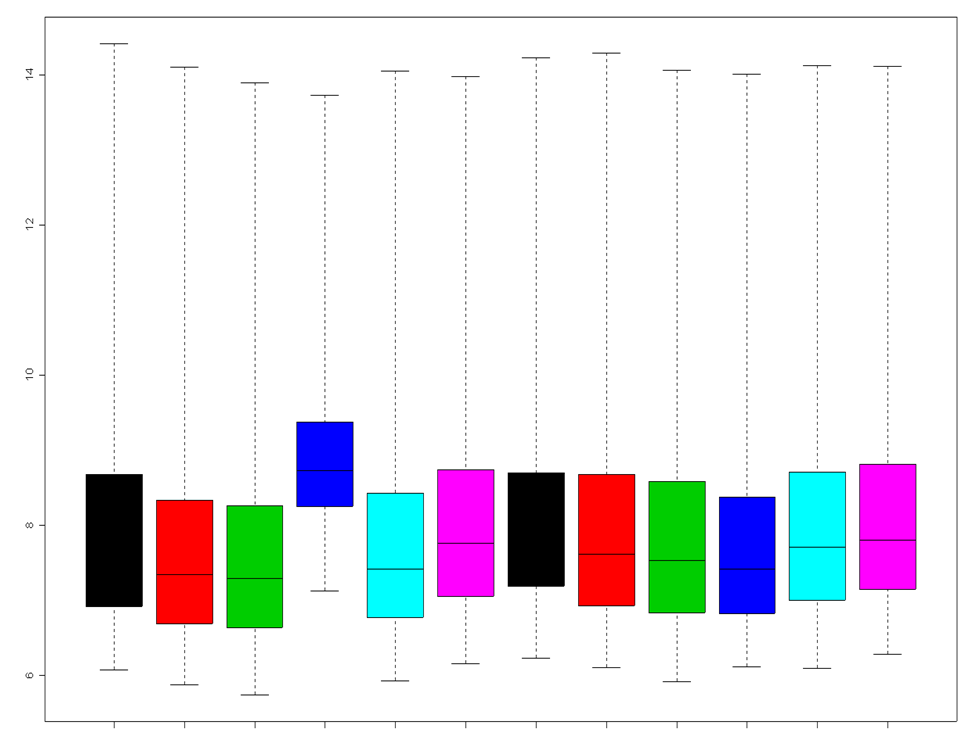
\includegraphics[scale=0.35]{pre_normalization.png}
\end{figure}
\end{itemize}
\end{frame}

\begin{frame}[fragile]{Procesando los Datos}
\textbf{Normalización}
\begin{itemize}
\item Ajustar las mediciones de los arreglos para que esten en la misma escala
\item Poder comparar las muestras
\begin{figure}[H]
\centering
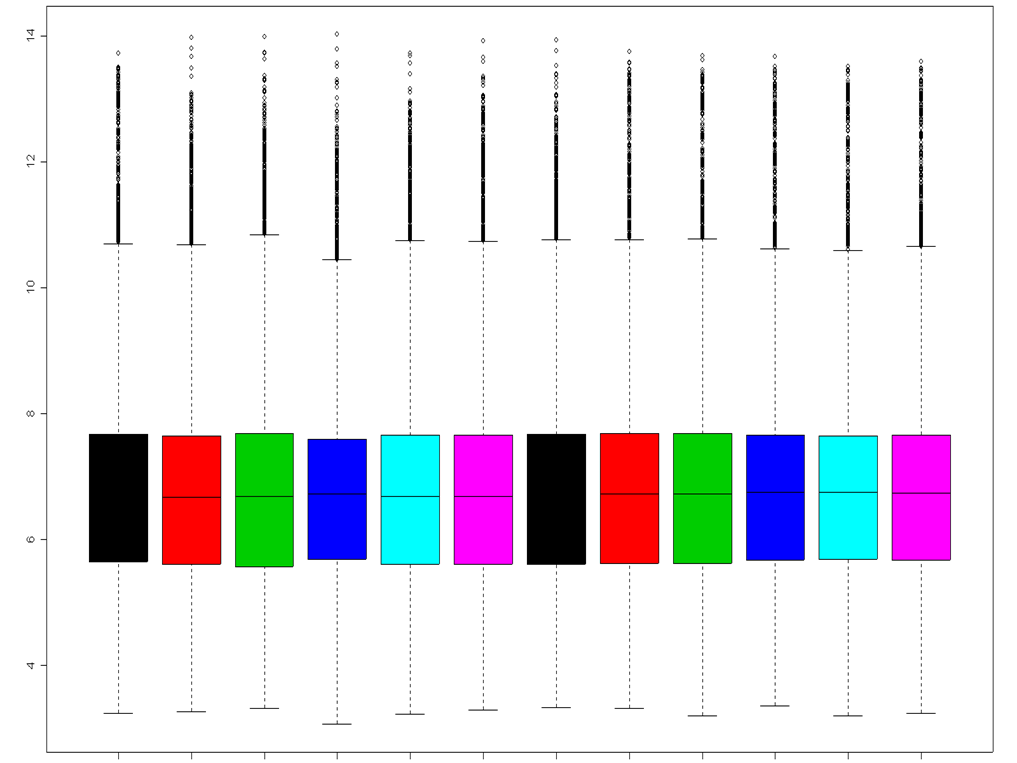
\includegraphics[scale=0.35]{post_normalization.png}
\end{figure}
\end{itemize}

\end{frame}

\begin{frame}[fragile]{Procesando los Datos}
\textbf{Resumen}
\begin{itemize}
\item Estimar el promedio de la intensidad por grupos de sondas
\end{itemize}
\begin{figure}[H]
\centering
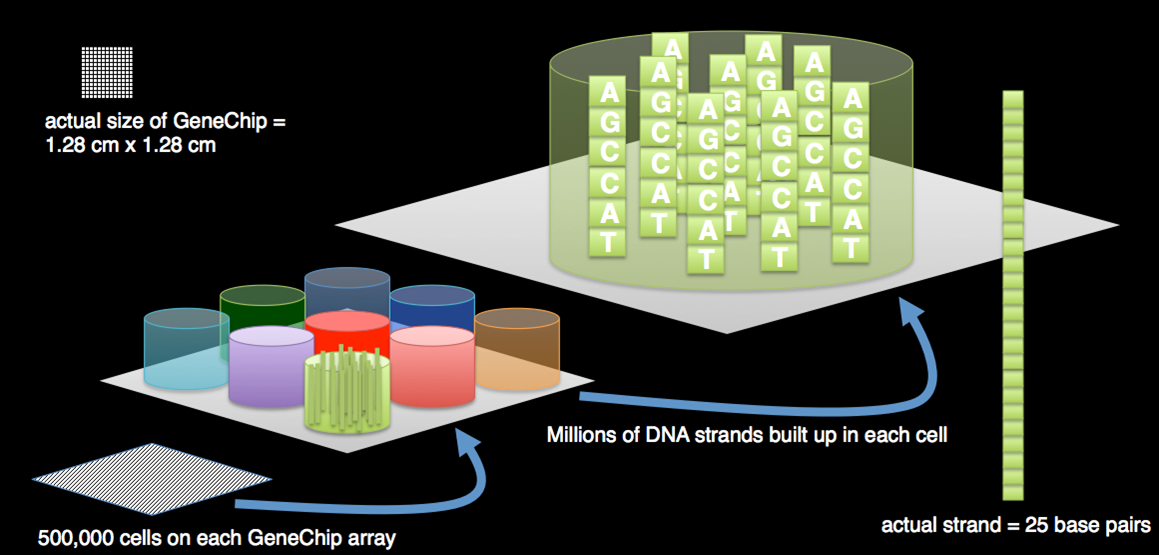
\includegraphics[scale=0.3]{affy00.png}
\end{figure}

\textbf{En R}
\begin{verbatim}
e <- rma(ab)
\end{verbatim}
\end{frame}

\begin{frame}[fragile]{Datos de Microarreglos}
\begin{itemize}
\item Hay varias formas de leer los datos de microarreglos
\item Ahora vamos a usar el paquete \verb=oligo=
\begin{verbatim}
detach("package:affy")
library(oligo)
\end{verbatim}
\item Repetir los pasos anteriores
\begin{verbatim}
basedir <- paste0(wd,"/celfiles")
setwd(basedir)
tab <- read.delim("sampleinfo.txt",check.names=FALSE,
				   as.is=TRUE)
\end{verbatim}
\item Revisar que tenemos todos los archivos
\begin{verbatim}
fns <- list.celfiles(listGzipped=TRUE)
fns %in% tab[,1]
\end{verbatim}
\end{itemize}
\end{frame}

\begin{frame}[fragile]{Datos de Microarreglos}
\begin{itemize}
\item Ingresar la información acerca de las muestras
\begin{verbatim}
pd <- as(tab, "AnnotatedDataFrame")
\end{verbatim}
\item Leer los archivos \verb=CEL=
\begin{verbatim}
efs <- read.celfiles(filenames=tab[,1],
		             phenoData=pd,sampleNames=sampleNames(pd))
\end{verbatim}
\item Procesar los datos
\begin{verbatim}
setwd(wd)
e <- rma(efs)
\end{verbatim}
\end{itemize}
\end{frame}

\begin{frame}{Anotación}
\begin{itemize}
\item ¿Dónde quedaron los genes?
\end{itemize}
\begin{figure}[H]
\centering
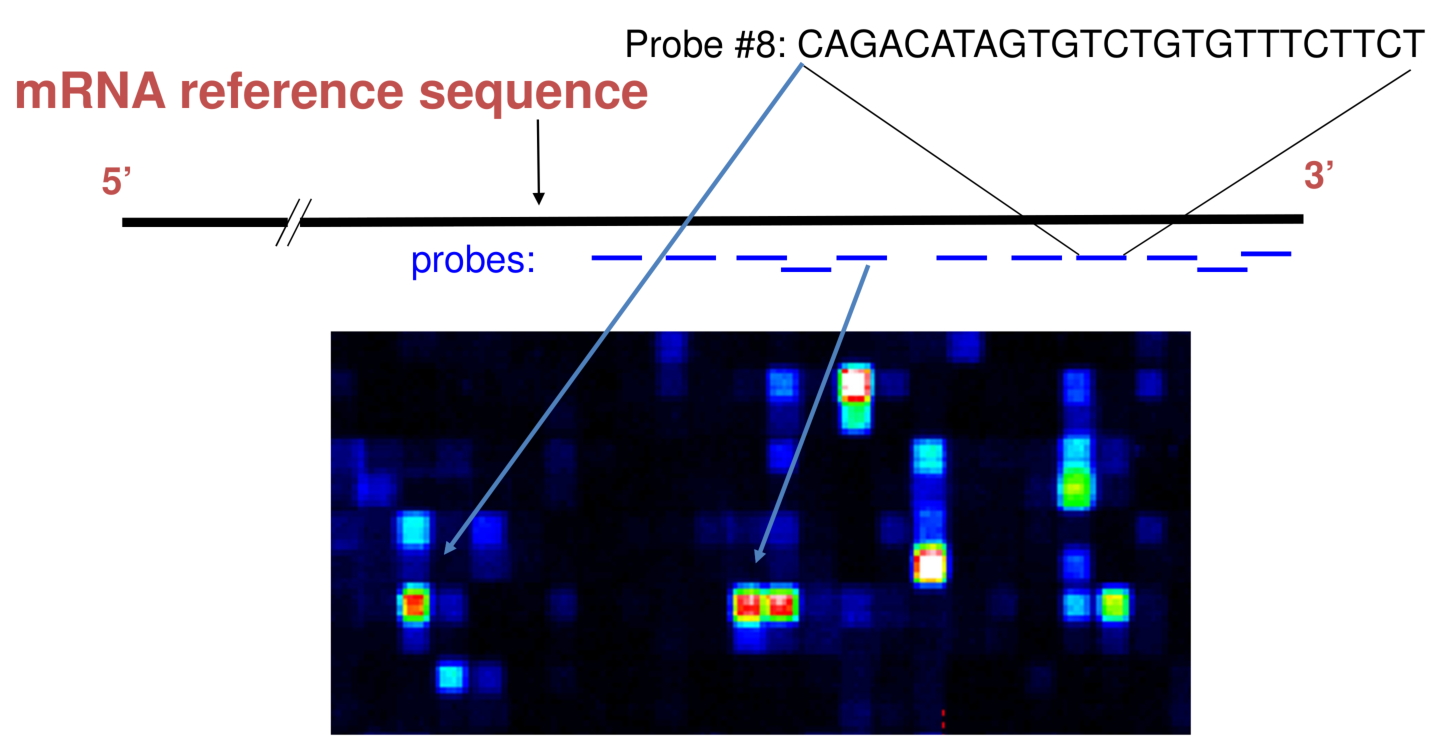
\includegraphics[scale=0.45]{affy_gene_exp.pdf}
\end{figure}
\end{frame}

\begin{frame}{Anotación}
\begin{itemize}
\item Anotación: que sondas corresponden a que genes
\end{itemize}
\begin{figure}[H]
\centering
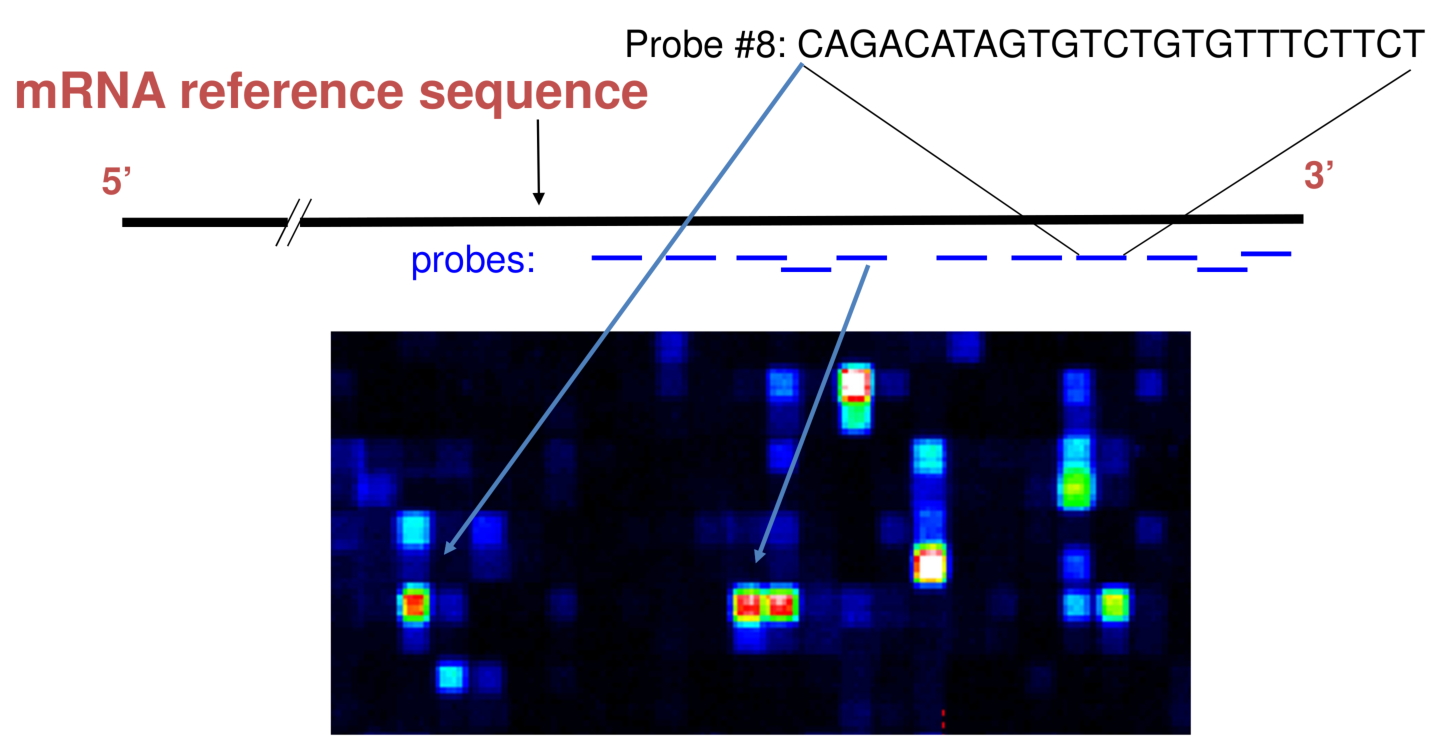
\includegraphics[scale=0.45]{affy_gene_exp.pdf}
\end{figure}
\end{frame}


\begin{frame}[fragile]{Anotación}
\begin{itemize}
\item Para este ejemplo vamos a usar los datos de \verb=maPooling=
\item Descarga el archivo \verb=maPooling.RData= en to working directory\\
\url{https://dl.dropboxusercontent.com/u/21912429/CdeC/maPooling.RData}
\item Los archivos \verb=RData= son archivos de R para guardar datos
\begin{verbatim}
library(Biobase)

load("maPooling.RData")
e <- maPooling
head(rownames(e))
\end{verbatim}
%\item Plataforma
%\begin{verbatim}
%annotation(e)
%\end{verbatim}
%\item Affymetrix Rat Expression Set 230 (\texttt{rae230a})
\end{itemize}
\end{frame}

\begin{frame}[fragile]{Anotación}
\begin{itemize}
\item Plataforma
\begin{verbatim}
annotation(e)
\end{verbatim}
\item Affymetrix Rat Expression Set 230 (\texttt{rae230a})
\end{itemize}
\begin{figure}[H]
\centering

\includegraphics[scale=0.2]{gangsta_rat.png}
\end{figure}
\end{frame}

\begin{frame}[fragile]{Anotación}
\begin{itemize}
\item Paquetes para anotación
\begin{verbatim}
library(rae230a.db)
library(AnnotationDbi)
\end{verbatim}
\item Campos disponibles
\begin{verbatim}
columns(rae230a.db)
\end{verbatim}
\item \verb=Keys=: campos que se pueden como palabras claves 
\begin{verbatim}
keytypes(rae230a.db)
\end{verbatim}
\item Por ejemplos, podemos usar los nombres de las sondas para acceder a los otros campos de la anotación
\begin{verbatim}
head(keys(rae230a.db, keytype="PROBEID"))
\end{verbatim}
\item En nuestas muestras
\begin{verbatim}
head(rownames(e))
\end{verbatim}
\end{itemize}
\end{frame}

\begin{frame}[fragile]{Anotación}
\textbf{Nombres de los Genes}
\begin{itemize}
\item Ensembl (European Bioinformatics Institute \& Wellcome Trust Sanger Institute)
\item Entrez (National Center for Biotechnology Information)
\item Symbol (Human Genome Organisation)
\begin{verbatim}
res <- select(rae230a.db, keys=rownames(e),
              columns=c("ENTREZID","ENSEMBL","SYMBOL"), 
              keytype="PROBEID")
			  
head(res)
\end{verbatim}
\end{itemize}
\end{frame}

\begin{frame}[fragile]{Anotación}
\begin{itemize}
\item Vamos a agregar esta información a nuestras muestras
\begin{verbatim}
idx <- match(rownames(e), res$PROBEID)
head(rownames(e))
head(res$PROBEID,7)
fData(e) <- res[idx,]
head(fData(e),10)
\end{verbatim}
\item Vamos a asegurarnos que los nombres corresponden
\begin{verbatim}
all.equal(fData(e)$PROBEID, rownames(e))
\end{verbatim}
\end{itemize}
\end{frame}



\begin{frame}[fragile]{GEO}
\begin{figure}[H]
\centering

\includegraphics[scale=0.45]{geo_main.png}
\end{figure}
\begin{itemize}
\item Gene Expression Omnibus (GEO)
\item Repositorio de datos genómicos del National Center for Biotechnology Information (NCBI)
\item Alrededor del 90\% de los datos son estudios de expresión genética
\item Los datos tienen 2 identificiones principalmente:
\begin{itemize}
\item GEO Sample (GSM)
\item GEO Series (GSE)
\end{itemize} 
\item Vamos a usar el paquete \verb=GEOquery= para descargar datos de GEO directamente a R
\end{itemize}
\end{frame}

\begin{frame}[fragile]{GEO}
\begin{itemize}
\item Datos procesados
\begin{verbatim}
library(GEOquery)
gse <- getGEO("GSE21653", GSEMatrix=TRUE)
show(gse)
\end{verbatim}
\item Archivos sin procesar: si los archivos \verb=.CEL= estan disponibles los podemos descargart usando la funcion \verb=getGEOSuppFiles=
\item Como argumento para esta funcion usamos una identificacion de GEO
\item Esta función crea un folder en el working directory para guardar los archivos sin procesar
\begin{verbatim}
filePaths = getGEOSuppFiles('GSE21653')
filePaths
\end{verbatim}
\end{itemize}
\end{frame}


\end{document}

\begin{frame}[fragile]{Anotación}
\end{frame}








